\subsection{Selection optimization}
\label{sec:eejjOptimization}    

The final event selection criteria are optimized by maximizing the expected signal significance defined as 
$S/\sqrt{S+B}$, where S (B) is the expected number of signal (background) events passing the 
selection requirements. Three variables (\st,~\mejmin, and \mee) are optimized 
simultaneously by scanning appropriate ranges of values.
For this study the \ttbar~MC is used, instead of the data-driven method 
described in Section~\ref{sec:eejjTTbarBkg}. 
The results of the optimization, obtained for each LQ mass hypothesis, 
are summarized in Table~\ref{tab:eejjOptimizedCuts} assuming an 
integrated luminosity of \lumi.
Figure \ref{fig:eejj-optimization} shows the smooth dependence of the 
optimized \mej~and \st~cut values on the leptoquark mass hypothesis.

\begin{figure}
  \begin{center}
    {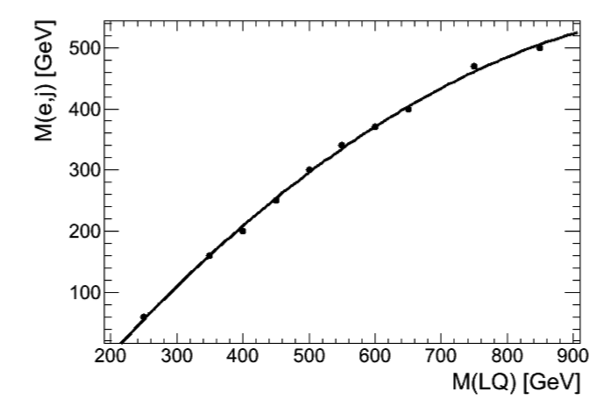
\includegraphics[width=.45\textwidth]{tex/analysis/event_selection/fig/optimization/optimization_eejj_mej.png}}
    {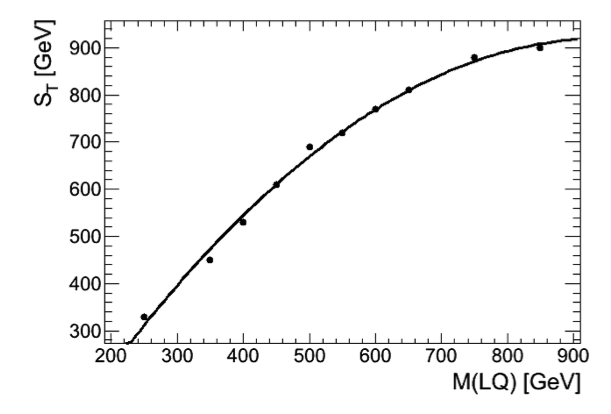
\includegraphics[width=.45\textwidth]{tex/analysis/event_selection/fig/optimization/optimization_eejj_st.png}}
    \caption{
      Optimized thresholds for for \mej~(left) and \st~(right) cuts
      as a function of leptoquark mass in the \eejj~channel.
      The leptoquark mass hypothesis under consideration is shown on the $x$-axis.
      The optimized cut thresholds are shown on the $y$-axis.
      The resulting distributions are fit with a second-degree polynomial.
    }
    \label{fig:eejj-optimization}
  \end{center}
\end{figure}

\begin{table}
  \begin{center}
    \begin{tabular}{ l | c | c | c | c | c | c | c | c | c | c | c } 
      \MLQ~[GeV]  & 250 & 350 & 400 & 450 & 500 & 550 & 600 & 650 & 750 & 850 & 900 \\ 
      \hline 
      \hline 
      \st~[GeV]  & 330 & 450 & 530 & 610 & 690 & 720 & 770 & 810 & 880 & 900 & 920 \\ 
      \hline 
      \mejmin~[GeV]  & 60 & 160 & 200 & 250 & 300 & 340 & 370 & 400 & 470 & 500 &  520 \\ 
      \hline 
      \mee [GeV] & 100 & 110 & 120 & 130 & 130 & 130 & 130 & 130 & 140 & 150 & 150 \\ 
    \end{tabular}   
    \caption{Optimized selection criteria for the \eejj~channel for different LQ mass hypotheses.}
    \label{tab:eejjOptimizedCuts}
  \end{center}
\end{table}
    
